\subsection{Run-length coding (RLC)}
\subsubsection*{Input}
The document need to compress.
\subsection*{Output}
The compressed document.
\subsubsection*{Basic idea}
Run-length encoding simple replaces sequences of the same data values within a file by a count number and a single value.
\subsubsection*{Example}
\paragraph*{}
Suppose the following string of data (17 bytes) has to be compressed: ABBBBBBBBBCDEEEEF
\paragraph*{}
Using RLE compression, the compressed file takes up 12 bytes and could look like this: 1A 8B 1C 1D 4E 1F
\paragraph*{}
And for decompression, all we need is "write down" exactly "count number" times for each symbol. Finally, the result would be the same:\\
ABBBBBBBBBCDEEEEF
\subsubsection*{Pseudo-code}
You can find pseudo-code (Python style) for Run-length encoding and decoding in \textit{pseudo-code/run-length.py}
\subsection{Shannon-Fano coding}
\subsubsection*{Input}
Set of symbol S.\\
The document need to compress.
\subsubsection*{Output}
The compressed document.\\
The table of frequency (or number of times symbol appears in the document).
\subsubsection*{Basic idea}
\begin{enumerate}
\item For a given list of symbols, calculate table of probabilities or frequency counts for the document
\item Sort the lists of symbols according to frequency (descending order)
\item Divide the list into two parts, with the total frequency counts of the left part being as close to the total of the right as possible.
\item The left part of the list is started with the code 0, and the right part is started with code 1. 
\item Recursively apply the steps 3 and 4 to each of the two halves, subdividing groups and adding bits to the codes until each symbol has become a corresponding code leaf on the tree.
\end{enumerate}
\pagebreak
\subsubsection*{Example}
The document need to compress: "ABBACAABCECAABADDDE".\\
Set of symbols S = {A, B, C, D, E}.\\
Encoded message: "0001010010000001101111000000100110110110111".\\
Decoded message: "ABBACAABCECAABADDDE".
\begin{table}[h!]
  \begin{center}
    \pgfplotstabletypeset[
      	multicolumn names,
      	col sep=comma,
      	string type,
      	display columns/0/.style={column name=$Symbol$, column type={c}},
      	display columns/1/.style={column name=$Count$, column type={S}},
      	display columns/2/.style={column name=$Probability$, column type={S}},
      	every head row/.style={before row={\toprule}, after row={\midrule}},
      	every row/.style={after row={\midrule}},
		every last row/.style={after row=\bottomrule},
    ]{tables/shannon.csv}
    \caption[Shannon-Fano exaple frequency]{Calculate the table of frequency (descending oder)}
  \end{center}
\end{table}
\begin{figure}[h!]
	\centering
	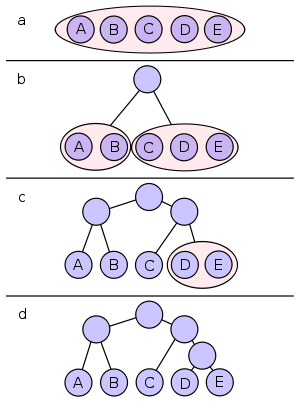
\includegraphics[width=0.5\linewidth]{images/shannon_fano_example.png}
	\caption[Shannon-Fano exaple tree]{Divide the list of symbols and assign code}
\end{figure}
\pagebreak
\begin{table}[h!]
  \begin{center}
    \pgfplotstabletypeset[
      	multicolumn names,
      	col sep=comma,
      	string type,
      	display columns/0/.style={column name=$Symbol$, column type={c}},
      	display columns/1/.style={column name=$Code$, column type={c}},
      	every head row/.style={before row={\toprule}, after row={\midrule}},
      	every row/.style={after row={\midrule}},
		every last row/.style={after row=\bottomrule},
    ]{tables/shannon-code.csv}
    \caption[Shannon-Fano exaple code]{The final code of symbols}
    \label{shannon-code}
  \end{center}
\end{table}
\subsubsection*{Pseudo-code}
You can find pseudo-code (Python style) for Shannon-Fano encoding and decoding in \textit{pseudo-code/shannon-fano.py}

\subsection{Lossless jpeg}
\subsubsection*{Input}
The input of jpeg usually is an image need to compress.
\subsubsection*{Output}
The compressed "image"
\subsubsection*{Basic idea}
For Compression:
\begin{enumerate}
\item Choose a predictor $P$.
\item Apply the predictor $P$ on the input image $I$ to get $I_p$ (the first pixel [0, 0] mustn't change).
\item Calculate the different image $I_d = I - I_p$.
\item Run a lossless compression algorithm on $I_d$ and get the compressed image.
\end{enumerate}
For decompression:
\begin{enumerate}
\item Run the lossless decompression (same with the 4th step above) we get $I_d$
\item Apply the predictor $P$ fro each pixel $p_i$ from the first pixel [0, 0] of $I_d$
\item Then sum up the value from step 2 with the value of $p_i$ in $I_d$ and we will pixel value of the original image.
\end{enumerate}
\subsubsection*{Examples}
Suppose we have a gray-scale image (4x4) $I$ like this:
\begin{equation*}
\begin{matrix}
90 & 92 & 89 & 70\\
75 & 65 & 67 & 69\\
90 & 92 & 89 & 70\\
90 & 92 & 89 & 70\\
\end{matrix}
\end{equation*}
Now, we apply the predictor $X = A + B - C$ to compute $I_p$:
\begin{equation*}
\begin{matrix}
90 & 90 & 92 & 89\\
90 & 77 & 62 & 48\\
75 & 65 & 82 & 83\\
75 & 75 & 89 & 93\\
\end{matrix}
\end{equation*}
Then, we have the different image $I_d$:
\begin{equation*}
\begin{matrix}
90 & 2 & -3 & -19\\
-15 & -12 & 5 & 21\\
0 & 15 & -1 & 4\\
-5 & 10 & 1 & -13\\
\end{matrix}
\end{equation*}
Finally, we can choose another lossless compressor to compress $I_d$.
\subsubsection*{Pseudo-code}
You can find pseudo-code (Python style) for Lossless jpeg encoding and decoding in \textit{pseudo-code/lossless-jpeg.py}
